\documentclass[10pt]{amsart}
\usepackage{amsmath}
\usepackage{amssymb}
\usepackage{amsthm}
%\usepackage{MnSymbol}
\usepackage{bm}
\usepackage{accents}
\usepackage{mathtools}
\usepackage{tikz}
\usetikzlibrary{calc}
\usetikzlibrary{decorations.pathmorphing,shapes,decorations.pathreplacing}
\usetikzlibrary{automata,positioning}
\usepackage{tikz-cd}
\tikzcdset{
  diagrams={>={Straight Barb[scale=0.5]}}
}

\tikzset{
    altstackar/.style={decorate, decoration={show path construction,
    lineto code={
      \path (\tikzinputsegmentfirst); \pgfgetlastxy{\xstart}{\ystart}
      \path (\tikzinputsegmentlast); \pgfgetlastxy{\xend}{\yend}
      \path ($(0,0)!1.5pt!(\ystart-\yend,\xend-\xstart)$); \pgfgetlastxy{\xperp}{\yperp}
      \foreach \n[evaluate=\n as \k using .5*#1-\n+.5] in {1,...,#1}{
        \ifodd\n{\draw[->, shorten <=2pt, shift={($\k*(\xperp,\yperp)$)}](\xstart,\ystart)--(\xend,\yend);}
        \else{\draw[<-, shorten >=2pt, shift={($\k*(\xperp,\yperp)$)}](\xstart,\ystart)--(\xend,\yend);}\fi
      }
    }
  }}, altstackar/.default={1}
}

\usepackage{forest}
\usepackage{braket} 
\usepackage{listings}
\usepackage{mdframed}
\usepackage{verbatim}
\usepackage{physics2}
\usephysicsmodule{ab,ab.legacy,diagmat,xmat,op.legacy}
\usepackage{derivative}
\usepackage{fixdif}
\usepackage{stmaryrd}
% \usepackage{euscript} 
\usepackage{eucal}
\usepackage{stackengine}
\usepackage{spectralsequences} 
%\usepackage{/home/patrickl/homework/macaulay2}

%font
% % \usepackage[sc]{mathpazo}
% \usepackage{inconsolata}
\usepackage{microtype}
\usepackage[lf]{ebgaramond}
\usepackage{inconsolata}
\usepackage[scaled]{helvet}
\usepackage[vvarbb,amsthm,ebgaramond,frenchmath,smallerops]{newtxmath}
% \usepackage{fontspec} 
% \setmainfont{Tex Gyre Pagella}
% \usepackage[OT1,euler-digits]{eulervm}
% \usepackage{euler-math} 
% \usepackage[scaled=0.86]{berasans}
% \let\sffamilyold\sffamily
% \def\sffamily{\fontencoding{T1}\sffamilyold}
% \setmonofont{Inconsolatazi4}

%CS packages
\usepackage{algorithmicx}
\usepackage{algpseudocode}
\usepackage{algorithm}

% typeset and bib
\usepackage[english]{babel} 
% \usepackage[utf8]{inputenc} 
% \usepackage[T1]{fontenc}
% \usepackage[backend=biber,style=alphabetic,maxalphanames=4,maxnames=5,hyperref,backref=true,backrefstyle=none]{biblatex}
\usepackage[bookmarks, colorlinks, breaklinks]{hyperref} 
\hypersetup{linkcolor=blue,citecolor=magenta,filecolor=black,urlcolor=blue}
\usepackage{cleveref}
\crefname{equation}{}{}
\usepackage{graphicx}
\graphicspath{{./}}
% \usepackage{xpatch}
% \xpatchbibmacro{pageref}{parens}{backrefparens}{}{}
% \DefineBibliographyStrings{english}{
%     backrefpage={$\leftarrow$},
%     backrefpages={$\leftarrow$},
% }
\usepackage{xcolor} 


% other formatting packages
\usepackage{float}
\usepackage{booktabs}
\usepackage[shortlabels]{enumitem}
\setitemize{noitemsep}
\usepackage{csquotes}
%\usepackage{titlesec}
%\usepackage{titling}
%\usepackage{fancyhdr}
%\usepackage{lastpage}
% \usepackage{parskip}
\newlist{mydescription}{description}{1}
\setlist[mydescription]{style=nextline,
                        font=\bfseries,
                        % Tweak the next 4 options as needed:
                        labelindent=1cm, 
                        leftmargin =2cm,
                        rightmargin=1cm,
                        topsep     =1ex
                       }

\usepackage{lipsum}

% delimiters
\DeclarePairedDelimiter{\gen}{\langle}{\rangle}
\DeclarePairedDelimiter{\floor}{\lfloor}{\rfloor}
\DeclarePairedDelimiter{\ceil}{\lceil}{\rceil}


\newtheorem{thm}{Theorem}[section]
\newtheorem{cor}[thm]{Corollary}
\newtheorem{prop}[thm]{Proposition}
\newtheorem{lem}[thm]{Lemma}
\newtheorem{conj}[thm]{Conjecture}
\newtheorem{quest}[thm]{Question}
\newtheorem{claim}[thm]{Claim}
\newtheorem{slog}[thm]{Slogan}

\theoremstyle{definition}
\newtheorem{defn}[thm]{Definition}
\newtheorem{defns}[thm]{Definitions}
\newtheorem{con}[thm]{Construction}
\newtheorem{exm}[thm]{Example}
\newtheorem{exms}[thm]{Examples}
\newtheorem{notn}[thm]{Notation}
\newtheorem{notns}[thm]{Notations}
\newtheorem{addm}[thm]{Addendum}
\newtheorem{exer}[thm]{Exercise}

\theoremstyle{remark}
\newtheorem{rmk}[thm]{Remark}
\newtheorem{rmks}[thm]{Remarks}
\newtheorem{warn}[thm]{Warning}
\newtheorem{sch}[thm]{Scholium}


% unnumbered theorems
\theoremstyle{plain}
\newtheorem*{thm*}{Theorem}
\newtheorem*{prop*}{Proposition}
\newtheorem*{lem*}{Lemma}
\newtheorem*{cor*}{Corollary}
\newtheorem*{conj*}{Conjecture}

% unnumbered definitions
\theoremstyle{definition}
\newtheorem*{defn*}{Definition}
\newtheorem*{exer*}{Exercise}
\newtheorem*{defns*}{Definitions}
\newtheorem*{con*}{Construction}
\newtheorem*{exm*}{Example}
\newtheorem*{exms*}{Examples}
\newtheorem*{notn*}{Notation}
\newtheorem*{notns*}{Notations}
\newtheorem*{addm*}{Addendum}


\theoremstyle{remark}
\newtheorem*{rmk*}{Remark}

% shortcuts
\newcommand{\Ima}{\mathrm{Im}}
\newcommand{\A}{\mathbb{A}}
\newcommand{\G}{\mathbb{G}}
\newcommand{\N}{\mathbb{N}}
\newcommand{\R}{\mathbb{R}}
\newcommand{\C}{\mathbb{C}}
\newcommand{\Z}{\mathbb{Z}}
\newcommand{\Q}{\mathbb{Q}}
\newcommand{\E}{\mathbb{E}}
\newcommand{\F}{\mathbb{F}}
\renewcommand{\k}{\Bbbk}
\renewcommand{\L}{\mathbb{L}}
\renewcommand{\P}{\mathbb{P}}
\newcommand{\M}{\mathcal{M}}
\newcommand{\Mbar}{\overline{\mathcal{M}}}
\newcommand{\g}{\mathfrak{g}}
\newcommand{\h}{\mathfrak{h}}
\newcommand{\n}{\mathfrak{n}}
\renewcommand{\b}{\mathfrak{b}}
\newcommand{\ep}{\varepsilon}
\newcommand*{\dt}[1]{%
   \accentset{\mbox{\Huge\bfseries .}}{#1}}
%\renewcommand{\abstractname}{Official Description}
\newcommand{\mc}[1]{\mathcal{#1}}
\newcommand{\T}{\mathbb{T}}
\newcommand{\mf}[1]{\mathfrak{#1}}
\newcommand{\mbf}[1]{\mathbf{#1}}
\newcommand{\bv}{\mbf{v}}
\newcommand{\bq}{\mbf{q}}
\newcommand{\bp}{\mbf{p}}
\newcommand{\ut}{\ul{t}}
\newcommand{\uz}{\ul{z}}
\newcommand{\ur}{\ul{j}}
\newcommand{\btau}{\bm{\tau}}
\newcommand{\mr}[1]{\mathrm{#1}}
\newcommand{\on}[1]{\operatorname{#1}}
\newcommand{\ms}[1]{\mathsf{#1}}
\newcommand{\mt}[1]{\mathtt{#1}}
\newcommand{\ol}[1]{\overline{#1}}
\newcommand{\ul}[1]{\underline{#1}}
\newcommand{\wt}[1]{\widetilde{#1}}
\newcommand{\wh}[1]{\widehat{#1}}
\renewcommand{\div}{\operatorname{div}}
\newcommand{\1}{\mathbf{1}}
\newcommand{\2}{\mathbf{2}}
\newcommand{\3}{\mathbf{3}}
\newcommand{\I}{\mathrm{I}}
\newcommand{\II}{\mr{I}\hspace{-1.3pt}\mr{I}}
\newcommand{\III}{\mr{I}\hspace{-1.3pt}\mr{I}\hspace{-1.3pt}\mr{I}}
\renewcommand{\v}{\mbf{v}}
\newcommand{\w}{\mbf{w}}
\newcommand{\bmu}{\bm{\mu}}
\newcommand{\pre}{\mr{pre}}
\newcommand{\vir}{\mr{vir}}
\newcommand{\red}{\mr{red}}
\newcommand{\pt}{\mr{pt}}
\newcommand{\tw}{\mr{tw}}
\newcommand{\fl}{\mr{fl}}
\newcommand{\ps}[1]{\llbracket #1 \rrbracket}
\newcommand{\ls}[1]{\llparenthesis #1 \rrparenthesis}
\newcommand{\dps}[1]{\ab<\!\ab< #1 >\!>}
\newcommand{\HN}{\ms{HC}^-}
\newcommand{\HC}{\ms{HC}}
\newcommand{\THH}{\ms{THH}}
\newcommand{\TC}{\ms{TC}}
\newcommand{\TP}{\ms{TP}}
\newcommand{\HH}{\ms{HH}}
\newcommand{\HP}{\ms{HP}}
\newcommand{\dR}{\ms{dR}}

\DeclareMathOperator{\Der}{Der}
\DeclareMathOperator{\Tor}{Tor}
\DeclareMathOperator{\Hom}{Hom}
\DeclareMathOperator{\RHom}{RHom}
\DeclareMathOperator{\End}{End}
\DeclareMathOperator{\Ext}{Ext}
\DeclareMathOperator{\ad}{ad}
\DeclareMathOperator{\Aut}{Aut}
\DeclareMathOperator{\Rad}{Rad}
\DeclareMathOperator{\Pic}{Pic}
\DeclareMathOperator{\NS}{NS}
\DeclareMathOperator{\supp}{supp}
\DeclareMathOperator{\Supp}{Supp}
\DeclareMathOperator{\depth}{depth}
\DeclareMathOperator{\sgn}{sgn}
\DeclareMathOperator{\spec}{Spec}
\DeclareMathOperator{\Spec}{Spec}
\DeclareMathOperator{\proj}{Proj}
\DeclareMathOperator{\Proj}{Proj}
\DeclareMathOperator{\ord}{ord}
\DeclareMathOperator{\Div}{Div}
\DeclareMathOperator{\Bl}{Bl}
\DeclareMathOperator{\coker}{coker}
\DeclareMathOperator{\ev}{ev}
\DeclareMathOperator{\st}{st}
\DeclareMathOperator{\pr}{pr}
\DeclareMathOperator{\ch}{ch}
\DeclareMathOperator{\Cont}{Cont}
\DeclareMathOperator{\Crit}{Crit}
\DeclareMathOperator{\op}{op}
\DeclareMathOperator{\Sym}{Sym} 
\DeclareMathOperator{\Tot}{Tot} 


\title{Topological cyclic homology}
\author{Patrick Lei}
\date{Spring 2025}
\allowdisplaybreaks
\setcounter{MaxMatrixCols}{12}

\begin{document}

\begin{abstract}
    These are notes taken live while watching the \href{https://www.youtube.com/playlist?list=PLsmqTkj4MGTB8pNGvW0iuKUFmBlOSke-C}{YouTube lectures} about topological cyclic homology by Thomas Nikolaus and Achim Krause. Note that we use homological grading throughout because the lecturers are homotopy theorists.
\end{abstract}
\maketitle
\tableofcontents

\section{Motivation: trace methods}%
\label{sec:Motivation}

One motivation to study topological cyclic homology is its relation to crystalline cohomology and syntomic cohomology in arithmetic geometry. However, this is very involved, so we will not discuss it in depth. We will instead discuss the original motivation, which are trace methods in algebraic K-theory.

Let $R$ be a ring. There is an invariant, called \textit{algebraic K-theory}, which produces groups $K_*(R)$ for all $* \geq 0$. These are very important, but are almost impossible to compute or to understand structurally. For example, even $K_*(\Z)$ is not very well-understood. They are known in all odd degrees, conjectured to vanish in degrees divisible by $4$ (this is equivalent to the Kummer-Vandiver conjecture in number theory). 

If you are a topologist, then one motivation is to study whether a retract $X$ of a finite CW complex is itself a finite CW complex. The obstruction to this lies in 
\[
    K_*(\Z[\pi_1(X)]).
\]
Another motivation is that by work of Whitehead and others (the $s$-cobordism theorem), the obstruction for a cobordism to be trivial lies in an algebraic K-theory group. There is now a higher version of this theorem which relates diffeomorphism groups to algebraic K-theory. A third motivation comes from the Baum-Connes conjecture, which has other applications in geometric topology. 

For other applications, the group $K_0$ was first invented by Grothendieck to give a statement of the Grothendieck-Riemann-Roch theorem, and algebraic K-theory is also related to special values of $L$-functions. 

\begin{defn}
    For a ring $R$, the group $K_0(R)$ is the Grothendieck group of isomorphism classes of finitely generated projective $R$-modules under the operation of direct sum.
\end{defn}

Higher $K$-groups are defined as homotopy groups of the space obtained by group completing the category of finitely-generated projective $R$-modules. This can be made precise using higher algebra and actually produces a spectrum, and then we can take its homotopy groups. We can see why this is so complicated. 

\begin{exm}
    It is easy to see that $K_0(\text{field}) = \Z$, but of course the higher $K$-groups are very complicated. Quillen computed them for finite fields, but if we leave this case this becomes extremely difficult. 
\end{exm}

\subsection{Approximation of algebraic K-theory}%
\label{sub:Approximation of algebraic K-theory}

We will attempt to approximate algebraic K-theory using more algebraic invariants. There is a \textit{Dennis trace map} to Hochschild homology. There are refinements of this which fit into a diagram
\begin{equation*}
\begin{tikzcd}
    K_*(R) \ar{dr}{\text{cyclotomic trace}} \\
    & \TC_*(R) \ar{r} \ar{d} & \HC_*^-(R) \ar{d} \\
    & \THH_*(R) \ar{r} & \HH_*(R)
\end{tikzcd}
\end{equation*}

\begin{slog}
    The cyclotomic trace is often close to an isomorphism.
\end{slog}

There are also relative K-groups $K_*(R, I)$ for any ideal $I \subseteq R$, which is simply the homotopy fiber of $K(R) \to K(R/I)$. There are also relative $\TC$ groups, which are defined in the same way. We can also define groups with coefficients like $K_*(R, \Z_p)$ and $\TC_*(R, \Z_p)$. 

\begin{thm}[Dundas-Goodwillie-McCarthy, Clausen-Matthew-Morrow]
    \begin{enumerate}
        \item If $I \subseteq R$ is a nilpotent ideal, then 
        \[ \on{cyctr} \colon K_*(R,I) \to \TC_*(R, I) \]
        is an isomorphism.
        \item If $R$ is commutative and $I$-complete, the same conclusion holds with $p$-adic coefficients. In other words, we have
        \[
            K_*(R, I, \Z_p) \cong \TC_*(R, I, \Z_p).
        \]
        \item If $R$ is $p$-complete, then 
        \[ \TC_*(R, \Z_p) \cong K_*^{\text{\'et}}(R, \Z_p). \]
    \end{enumerate}
\end{thm}

\subsection{Why the trace map is a trace}%
\label{sub:Why the trace map is a trace}

Let $k$ be a field, $R$ be a $k$-algebra, and $P$ be a finitely generated projective right $R$-module. Then we have
\[ \Hom_R(P, P) \cong P \otimes_R \Hom_R(P, R). \]
We would attempt to go to $R$ by an evaluation map
\[ P \otimes_R \Hom_R(P, R) \xrightarrow{\ev} R, \]
but this doesn't actually land in $R$. Instead, we see that
\begin{align*}
    x \otimes r \varphi &\mapsto r \cdot \varphi(x) \\
    xr \otimes \varphi \mapsto \varphi(xr) = \varphi(x) \cdot r.
\end{align*}
The best we can do is to consider the quotient
\[ R / [R,R] \]
as an abelian groups, so in conclusion we have
\[ \tr \colon \Hom_R(P, P) \to R/[R,R]. \]

Note that an $R$-$R$-bimodule is equivalently an $R \otimes_k R^{\op}$-module. Then, we in fact have
\[ R/[R,R] \cong R \otimes_{R \otimes_k R^{\op}} R. \]
Deriving this expression, we will see later that
\[ \HH(R, k) \cong R \otimes^{\L}_{R \otimes_k R^{\op}} R. \]
The Dennis trace will refine this trace in the sense that on $K_0$, it will send a projective module $P$ to the trace of the identity endomorphism.

\section{Classical Hochschild and cyclic homology}%
\label{sec:Classical Hochschild and cyclic homology}

In this section, we discuss Hochschild homology, (negative, periodic) cyclic homology, the HKR theorem, and related topics.

\subsection{Hochschild homology}%
\label{sub:Hochschild homology}

Let \(k\) be a field and \(R\) be a \(k\)- algebra.

\begin{defn}
    The \textit{Hochschild homology} of \(R\) is the homology of the complex
    \[
        \HH(R/k) \coloneqq (\cdots \xrightarrow{\partial} R \otimes_k R \xrightarrow{\partial} R),
    \]
    where the differential is given by
    \begin{align*}
        \partial(a_0 \otimes \cdots \otimes a_n) \coloneqq{} & a_0 a_1 \otimes \cdots \otimes a_n \\
        &- a_0 \otimes a_1 a_2 \otimes \cdots \otimes a_n \\
        & \cdots \\
        &+ (-1)^n a_n a_0 \otimes \cdots \otimes a_{n-1}.
    \end{align*}
\end{defn}

\begin{rmk}
    This seems related to what happens when you multiply elements placed on an \(S^1\) as in~\Cref{fig:hhcircle}. In fact, we will see later that there is a connection to the actual \(S^1\).
    \begin{figure}[htpb]
    \begin{center}
    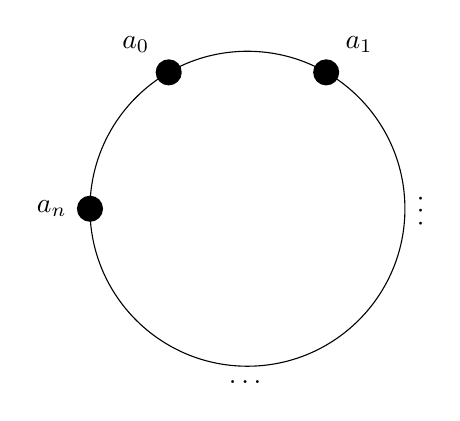
\begin{tikzpicture}[scale=1, transform shape]
        \draw (0,0) circle (2);
        \node[label={north west:{$a_0$}}, fill=black, circle] at (120:2) {};
        \node[label={north east:{$a_1$}}, fill=black, circle] at (60:2) {};
        \node[label={west:{$a_n$}}, fill=black, circle] at (180:2) {};
        \node[rotate=90] at (2.2,0) {\dots};
        \node at (0,-2.2) {\dots};
    \end{tikzpicture}
    \end{center}
    \caption{Components of a basic tensor placed along a circle.}%
    \label{fig:hhcircle}
    \end{figure}
\end{rmk}

\begin{exm}
    For now, set \(R=k\). In this case, we have
    \begin{align*}
        \HH(k/k) &= (\cdots \to k \to k),
    \end{align*}
    where the differentials are alternating sums of $1$ and $-1$. In fact, we see that the complex is
    \[ \HH(k/k) = (\cdots \xrightarrow{0} k \xrightarrow{\mr{id}} k \xrightarrow{0}k), \]
    and therefore the Hochschild homology is
    \[ \HH_*(k/k) = \begin{cases}
        k & *=0 \\
        0 & \text{otherwise}.
    \end{cases} \]
\end{exm}

\begin{exm}
    Because the last differential is given by $a \otimes b \mapsto ab - ba$, we see that
    \[ \HH_0(R/k) = R/[R,R]. \]
    In particular, if $R$ is commutative, we have
    \[ \HH_0(R/k) = R. \]
    In this case, we have
    \[ \HH_1(R/k) = \frac {R \otimes_k R}{\Im \partial} \cong \Omega^1_{R/k}. \]
\end{exm}

We will now recall the definition of the module of K\"ahler differentials.
\begin{defn}
    The \textit{module of K\"ahler differentials} of a commutative ring $R$ is the module $\Omega^1_{R/k}$ generated by $\d{x}$ for all $x \in R$ subject to the following relations:
    \begin{enumerate}
        \item For all $x, y \in R$, we have $\d{(x+y)} = \d{x} + \d{y}$;
        \item For all $x,y \in R$, we have $\d{(xy)} = x \d{y} + y \d{x}$;
        \item For all $x \in k$, we have $\d{x} = 0$.
    \end{enumerate}
    Therefore, we see that $\Omega^1_{R/k}$ receives a universal $k$-linear derivation from $R$.
\end{defn}

There is at most one map
\[ \HH_1(R/k) \to \Omega^1_{R/k} \qquad x \otimes y \mapsto x \cdot \d{y}. \]
\begin{exer}
    Check that this is an isomorphism.
\end{exer}

We will now prove some more properties of Hochschild homology.
\begin{lem}
    If $R$ is commutative, then \(\HH_*(R)\) has the structure of a strictly graded-commutative ring. Here, this means that \(x^2 = 0\) for any \(x\) of odd degree, which is only relevant in characterisic $2$.
\end{lem}

\begin{proof}
    The Hochschild complex $\HH(R/k)$ in fact comes from a simplicial commutative ring
    \begin{equation*}
    \begin{tikzcd}
        \cdots \ar[r,altstackar=7] & R \otimes_k \otimes_k R \ar[r,altstackar=5] & R\otimes_k R \ar[r,altstackar=3] & R,
    \end{tikzcd}
    \end{equation*}
    where the face maps are the components of the differential $\partial$. The desired result then follows by~\Cref{thm:eilenbergzilber}.
\end{proof}

On the de Rham side, there is also a multiplicative structure.
\begin{defn}
    The \textit{de Rham complex} is the exterior algebra
    \begin{align*}
        \Omega^*_{R/k} &\coloneqq \Lambda_R^* \Omega^1_{R/k} \\
        &= \bigoplus_{k \geq 0} \Lambda_R^k \Omega^1_{R/k} \\
        &= \frac{\Sym_R \Omega^1_{R/k}[1]}{x^2 = 0, x \in \Omega^1_{R/k}}.
    \end{align*}
\end{defn}

By extending from degree $1$, we obtain a map $\Omega^*_{R/k} \to \HH_*(R/k)$.

\begin{thm}[Hochschild-Kostant-Rosenberg]\label{thm:hkr}
    If $R/k$ has cotangent complex concentrated in degree $0$, then the map
    \[ \Omega^*_{R/k} \to \HH_*(R/k) \]
    is an isomorphism.
\end{thm}

We will discuss the cotangnet complex later, but for now we may think that $R$ is a smooth or ind-smooth $k$-algebra.

\begin{rmk}
    The differential on $\Omega^*_{R/k}$ does not play a role here. Studying what it corresponds to on the Hochschild side will leade us to cyclic homology.
\end{rmk}

\begin{exer}
    Find an explicit description of $\Omega^*_{k[x_1, \ldots, x_n]/k}$ and in particular show that it is concentrated in degrees at most $n$.
\end{exer}

We will now extend to the case when $k$ is an arbitrary commutative ring. This will lead to flatness issues, so we will fix this by taking derived tensor products. For now, we will let $R$ be a dg-algebra over $k$ which is $K$-flat. This is a flatness condition, but when $R$ is bounded below, it agrees with levelwise flatness. Over $\Z$, it always agrees with levelwise flatness. For such an $R$, we define the Hochschild complex by
\[ \HH(R/k) \coloneqq \Tot(\cdots \to R \otimes_k R \to R). \]
If $R$ is not $K$-flat, we will simply replace it by a $K$-flat resolution $R^{\flat}$ and define
\[ \HH(R/k) \coloneqq \HH(R^{\flat}.k). \]
This is well-defined up to quasi-isomorphism.

\begin{prop}
    For a dg-algebra $R$, there is a quasi-isomorphism
    \[ \HH(R/k) \simeq R \otimes_{R \otimes_k^{\L} R^{\mr{op}}}^{\L} R. \]
\end{prop}

\begin{rmk}
    This is usually called Shukla homology, but we will not make this distinction here.
\end{rmk}

\begin{proof}
    Replacing $R$ by a flat resolution, we consider the complex
    \[ \Tot(\cdots \to R \otimes_k R \otimes_k R \to R \otimes_k R) \simeq R. \]
    The differentials are given by multiplying adjacent terms, but without the $a_n a_0$ term (think configurations on an interval). This complex is usually called the \textit{bar complex}. Applying $- \otimes_{R \otimes_k R^{\op}} R$, the resulting total complex computes the desired complex $R \otimes_{R \otimes_k R^{\op}}^{\L} R$, but it also computes $\HH_*(R/k)$.
\end{proof}

\begin{lem}
    If $R$ is a dg-algebra which arises from a simplicial commutative $k$-algebra, then $\HH(R/k)$ also comes from a simplicial commutative $k$-algebra. In particular, the Hochschild homology groups $\HH_*(R/k)$ form a strictly graded-commutative $k$-algebra.
\end{lem}

\begin{proof}
    We replace $R$ by a flat simplicial commutative $k$-algebra. Applying Hochschild homology, then $\HH(R_n/k)$ gives a \textbf{bisimplicial} commutative $k$-algebra. The total complex is then quasi-isomorphic to the diagonal, which is clearly simplicial.
\end{proof}

\begin{lem}
    If $A, B$ are dg-algebras, then
    \[ \HH(A \otimes^{\L} B/k) \simeq \HH(A/k) \otimes_k^{\L} \HH(B/k). \]
\end{lem}

\begin{rmk}
    If $R$ is commutative, then setting $A=B=R$ gives a multiplication map on $\HH$ via the multiplication of $R$.
\end{rmk}

\begin{proof}
    Because $\HH(A/k)$ and $\HH(B/k)$ are simplicial dg-algebras, the tensor product
    \[ \HH(A/k) \otimes_k^{\L} \HH(B/k) \]
    is a bisimplicial dg-algebra. Taking the total complex in all three directions, the result is quasi-isomorphic to the diagonal, which is precisely
    \[ \HH(A\otimes_k^{\L} B). \qedhere \]
\end{proof}

We are now ready to prove the HKR theorem for polynomial rings. As we will see later, we will reduce the general case to this one.
\begin{proof}[Proof of~\Cref{thm:hkr} for polynomial rings]
    In the case of $R = k[x]$, we have
    \[ \Omega^*_{k[x]/k} = k[x] \otimes \Lambda(\d{x}). \]
    Then we only need to check that $\HH(k[x]/k)$ vanishes in degree greater than $1$. This is given by
    \begin{align*}
        \HH(k[x]/k) &= k[x] \otimes^{\L}_{k[x] \otimes_k k[x]} k[x] \\
        &= k[x] \otimes_{k[a,b]}^{\L} k[x].
    \end{align*}
    We have the resolution
    \[ k[a,b] \xrightarrow{\cdot (a-b)} k[a,b] \]
    of $k[x]$, and this gives the desired result.

    For \(R = k[x_1, \ldots, x_n]\) This is simply a tensor product
    \[ R = k[x_1] \otimes_k \cdots \otimes_k k[x_n], \]
    so because both sides of the HKR theorem commute with tensor products, we obtain the desired result.

    Finally, if \(R = k[x_i \mid i \in I]\), we write \(R\) as a filtered colimit of finitely-generated polynomial algebras by writing the set $\ab\{x_i \mid i \in I\}$ of generators as a filtered colimit of its finite subsets. Because both sides commute with filtered colimits, we are done.
\end{proof}

We will now turn to an extremely non-smooth example.
\begin{prop}
    We have
    \[ \HH_*(\F_p/\Z) = \F_p \ab<x>, \]
    where the $\ab<x>$ means the free divided power algebra generated by $x$.
\end{prop}

\begin{proof}
    We will compute the derived tensor product
    \[ \F_p \otimes_{\F_p \otimes^{\L} \F_p} \F_p. \]
    We will resolve $\F_p$ by the dg-algebra
    \[ \Z[\ep]/\ep^2, \qquad \partial \ep = p, \qquad \ab|\ep| = 1. \]
    The tensor product is then given by
    \[ A \simeq \F_p \otimes^{\L} \F_p \simeq \F_p[\ep]/\ep^2. \]
    We will resolve $\F_p$ as an $A$-algebra by
    \[ A\ab<x> = \frac{A[x_1, x_2, \ldots]}{x_ix_j = \binom{i+j}{i} x_{i+j}}, \qquad \partial x_i = \ep x_{i-1}, \qquad \ab|x_i| = 2i, \]
    and the desired result follows by taking the tensor product.
\end{proof}

\subsection{The Connes operator}%
\label{sub:The Connes operator}

We will describe an operator on $\HH$ which corresponds to the de Rham differential. Recall that the de Rham differential
\[ \d \colon \Omega^*_{R/k} \to \Omega^{*+1}_{R/k} \]
is induced from the universial derivation $\d \colon R \to \Omega^1_{R/k}$ by the Leibniz rule.

\begin{defn}
    Let $R$ be an associative $k$-algebra. We define a $k$-linear map
    \[ B \colon \HH(R/k)_n \to \HH(R/k)_{n+1} \]
    by the formula
    \[ r_0 \otimes \cdots \otimes r_n \mapsto \sum_{\sigma \in C_{n+1}} (-1)^{n\sigma(0)} (1 \otimes r_{\sigma} + (-1)^n r_{\sigma} \otimes 1), \]
    where we define
    \[ r_{\sigma} \coloneqq r_{\sigma(0)} \otimes \cdots \otimes r_{\sigma(n)}. \]
\end{defn}
This formula is related to the \textit{cyclic objects} introduced by Connes, and there is a way to think about it systematically in the topological setting, which we will discuss later.

\begin{exer}
    Check that
    \begin{enumerate}
        \item $B^2 = 0$;
        \item $\d B + B \d = 0$.
    \end{enumerate}
\end{exer}

The operator $B$ equips $\HH(R/k)$ with the structure of a dg-module over the dg-algebra
\[ A \coloneqq k[b]/b^2, \qquad \ab|b| = 1, \qquad \partial = 0. \]
Note that if $\T = U(1)$ is the circle group, then we have
\[ A = H_*(\T, k). \]
We then see that $\HH_*(R/k)$ is a graded module over $k[b]/b^2$, and in particular that there is an operator
\[ B \colon \HH_*(R/k) \to \HH_{*+1}(R/k) \]
satisfying $B^2 = 0$.

\begin{warn}
    One might object that we only defined the Connes operator only for algebras concentrated in degree $0$, but with some careful thought we can define $B$ for dg-algebras $R/k$.
\end{warn}

We need the following fact.
\begin{lem}
    If $R$ is commutative, then $B$ is a derivation. In particular, it satisfies the graded Leibniz rule
    \[ B(xy) = B(x) y + (-1)^{\ab|x|} x B(y). \]
\end{lem}

\begin{warn}
    The Connes operator is not true on the complex $\HH(R/k)$. It is true up to coherent homotopy, but proving this is very hard. Instead, we will later use the topological enhancement to understand this.
\end{warn}

\begin{prop}
    The map 
    \[ \Omega^*_{R/k} \to \HH_*(R/k) \]
    sends the de Rham differential $\d$ to the Connes operator $B$. In other words, the diagram
    \begin{equation*}
    \begin{tikzcd}
        \Omega^*_{R/k} \ar{r} \ar{d}{\d} & \HH_*(R/k) \ar{d}{B} \\
        \Omega^{*+1}_{R/k} \ar{r} & \HH_{*+1}(R/k)
    \end{tikzcd}
    \end{equation*}
    commutes.
\end{prop}

\begin{proof}
    The map $\Omega^*_{R/k} \to \HH_*(R/k)$ is determined by its effect in degrees $0$ and $1$. In degree $0$, it is given by the identity
    \[ R \to \HH_0(R/k) = R, \]
    and in degree $1$, it is given by
    \[ \Omega^1_{R/k} \to \HH_1(R/k) = \frac{R \otimes_k R}{\sim} \qquad x \d{y} \mapsto [x \otimes y]. \]
    Therefore, it is enough to check that the diagram
    \begin{equation*}
    \begin{tikzcd}
        R = \Omega^0_{R/k} \ar{r} \ar{d}{\d} & \HH_0(R/k) \ar{d}{B} \\
        \Omega^1_{R/k} \ar{r} & \HH_*(R/k)
    \end{tikzcd}
    \end{equation*}
    commutes. Note that for any $r \in R$, we see that all signs in the definition of $B$ are $+1$, so we have
    \[ B(r) = [1 \otimes r] + [r \otimes 1]. \]
    This corresponds to the element
    \[ 1 \cdot \d{r} + r \cdot d{1} = \d{r} \in \Omega^1_{R/k}. \]
    We conclude by using the fact that the de Rham differential is uniquely determined by being a derivation and its effect on $R$.
\end{proof}

\begin{rmk}
    Sometimes in the rest of these notes, we will denote the Connes operator by $\d$. If this causes confusion, we will call it $B$.
\end{rmk}

\begin{exm}
    For $\HH_*(\F_p/\Z) = \F_p \ab<x>$ with $x$ in degree $2$, the Connes operator acts trivially for degree reasons.
\end{exm}

\begin{quest}
    Does this mean that it acts trivially (maybe up to homotopy or quasi-isomorphism) on $\HH(\F_p, \Z)$?
\end{quest}

The answer to this question is in fact \textbf{no}, and we will see this by taking a (derived) reduction mod $p$. This means that we will consider
\[ \HH(\F_p) \sslash p \coloneqq \HH(F_p) \otimes_{\Z}^{\L} \F_p. \]
Letting $A$ act trivially on $\F_p$, we obtain a structure of an $A$-module on $\HH(\F_p) \sslash p$. We compute
\begin{align*}
    \HH(\F_p) \sslash p &\simeq \HH(F_p) \otimes_{\Z} (\Lambda_{\Z}(\ep), \ab|\ep| = 1, \partial \ep = p) \\
    &\simeq \HH(\F_p) \otimes_{\F_p} \Lambda_{\F_p}(\ep).
\end{align*}
This implies that
\begin{align*}
    H_* (\HH(\F_p) \sslash p) &\simeq \HH_*(\F_p) \otimes_{\F_p} \Lambda_{\F_p}(\ep) \\
    &\simeq \F_p \ab<x> \otimes_{\F_p} \Lambda_{\F_p}(\ep).
\end{align*}
\begin{prop}
    Writing the divided power $\gamma_n(x)$ as $x^{[n]}$, we have $B(x^{[n]}) = 0$ and $B(\ep) = x$.
\end{prop}
Note that this implies that 
\[ B(\ep x^{[n]}) = x x^{[n]} = (n+1)x^{[n+1]}. \]

\begin{proof}
    The map $\HH(\F_p) \to \HH(\F_p) \sslash p$ is compatible with $B$, and therefore we obtain $B(x^{[n]}) = 0$ in homology.

    Now recall that we computed
    \[ \HH_*(\F_p) = \F_p\ab<x> \]
    by replacing $\F_p$ by $(\Lambda_{\Z}(\ep), \partial \ep = p)$, so we write the complex
    \[ \cdots \xrightarrow{\partial} \Lambda_{\Z}(\ep) \otimes \Lambda_{\Z} (\ep) \xrightarrow{\partial} \Lambda_{\Z}(\ep). \]
    Writing out the full double complex, we obtain
    \begin{equation*}
    \begin{tikzcd}
        &\cdots \ar{r} & 0 \ar{r} \ar{d} & 0 \ar{d} \\
        &\cdots \ar{r} \ar{d} & \Z(\ep \otimes \ep) \ar{r} \ar{d}{(-p,p)} & 0 \ar{d} \\
        &\cdots \ar{r} \ar{d} & \Z(\ep \otimes 1) \oplus \Z(1 \otimes \ep) \ar{r}{0} \ar{d}{(p,p)}& \Z \ep \ar{d}{p} \\
        {}\ar{r}&\Z \ar[equals]{r} & \Z \ar{r}{0} & \Z.
    \end{tikzcd}
    \end{equation*}
    The class $x$ is given by $1 \otimes \ep - \ep \otimes 1$. Applying $B$, we obtain
    \[ B(\ep) = 1 \otimes \ep - \ep \otimes 1. \]
    After reducing mod $p$, we can replace all copies of $\Z$ by $\F_p$ and $\ep$ becomes a cycle, and we obtain $B(\ep) = x$.
\end{proof}

\subsection{Periodic and cyclic homology}%
\label{sub:Periodic and cyclic homology}

In the anology between Hochschild homology and the de Rham complex, we will now discuss cyclic homology, which will be analogous to algebraic de Rham cohomology.

We will work with derived functors in the category $\ms{DGMod}_A$. The homotopy theory we will work with is inverting quasi-isomorphisms, which means we will consider the $\infty$-category
\[ \ms{Mod}_A(D(k)). \]

\begin{defn}
    Let $R$ be a $k$-algebra.
    \begin{enumerate}
        \item The \textit{cyclic homology} of $R$ is
        \[ \HC_*(R/k) \coloneqq H_*(k \otimes_A^{\L} \HH(R/k)) = \Tor_*^A(k, \HH(R/k)). \]
        This will not play any role in these notes.
        \item The \textit{negative cyclic homology} of $R$ is
        \[ \HC_*^-(R/k) \coloneqq \RHom_A(k, \HH(R/k)) = \Ext_A^{-*}(k, \HH(R/k)). \]
        This is more important than cyclic homology, and topological cyclic homology will be an analog of this rather than of cyclic homology. Also, note that $\HC_*^-(R/k)$ is a module over $\Ext_A^{*}(k,k) = k[t]$, where $\ab|t| = -2$.
        \item The \textit{periodic cyclic homology} (or \textit{periodic homology}) of $R$ is
        \[ \HP_*(R/k) = \HC_*^-(R/k) [t^{-1}]. \]
    \end{enumerate}
\end{defn}

\begin{exer}
    Show that $\Ext_A^*(k,k) \cong k[t]$, where $\ab|t| = -2$.
\end{exer}

Note that the definition we gave is not the standard one in the literature, which involves double complexes. We may wonder if these definitions are equivalent.

\begin{prop}
    For any $k$-algebra $R$, we have
    \[ \HC^-(R/k) \simeq (\HH(R/k)\ps{t}, \partial + tB), \]
    where $\partial + tB$ is defined as
    \[ xt^i \mapsto (\partial x) t^i + (Bx) t^{i+1} \]
    for $x \in \HH(R/k)$ (this is basically saying that $\partial(t) = 0$). Moreover, we have
    \[ \HP(R/k) \simeq (\HH(R)\ls{t}, \partial + tB). \]
\end{prop}

\begin{proof}
    We will resolve $k$ as an $A$-algebra by
    \[ C = A\ab\{ x_0, x_1, \ldots\}, \qquad \ab|x_k| = 2k, \]
    where we declare that
    \[ \partial(x_k) = b x_{k-1}. \]
    Note that $C$ also has the structure of a coalgebra with coproduct given by
    \[ \Delta(x_k) = \sum_{i+j = k} \sum_{i+j=k} x_i \otimes x_j. \]
    This implies that
    \begin{align*}
        \RHom_A(k, \HH(R/k)) &= \ul{\Hom}_A(C, \HH(R/k)) \\
        &= (\HH(R/k)\ps{t}, \partial + tB).
    \end{align*}
    Here, we use the fact that $t^i$ is the dual of the element $x_i$, and therefore because the differential on $C$ is just $b$ and lowers the $x$-degree by $1$, dually it will be $B$ and raise the $t$-degree by $1$. The formula for $\HP(R/k)$ follows by inverting $t$.
\end{proof}

\begin{rmk}
    This argument works more generally to obtain $\RHom(k, H)$ for an arbitrary $H \in \ms{DGMod}_A$.
\end{rmk}

\begin{rmk}
    $A$ is a Hopf algebra with couint
    \[ \ep \colon A \to k \qquad \ep(b) = 0 \]
    and coproduct $\Delta \colon A \to A \otimes A$ given by
    \[ \Delta(b) = 1 \otimes b + b \otimes 1. \]
    This implies that $\ul{\RHom}_A(k, -)$ is a lax symmetric monoidal functor (here, note that $k$ is the unit in the category of dg $A$-modules) and as such is given by
    \[ H \mapsto (H \ps{t}, \partial + tB) \]
    as a lax symmetric monoidal functor. Moreover, if $C$ is an algebra object in $\ms{DGMod}_A$, i.e. $C$ is a dg algebra and $B$ satisfies the Leibniz rule, then $\ul{\RHom}_A(k, C)$ is a dg algebra.
\end{rmk}

\begin{warn}
    Even if $R$ is commutative, $B$ is \textbf{not} a derivation on $\HH(R)$, so we cannot simply argue that negative cyclic and periodic homology have products. This is true up to chain homotopy, however, but this is still not enough to obtain a product. We will see that $B$ is a derivation up to coherent homotopy, but we run into issues with the formality of $A$, which will require working with $S^1$ to resolve.

    Instead of doing all of that, we will use the hack that $(\HH(R/k)\ps{t}, \partial + tB)$ has a product up to chain homotopy. This implies that $\HC_*^-(R/k)$ and $\HP_*(R/k)$ are graded commutative algebras.
\end{warn}

Our goal now is to enhance the HKR theorem (\Cref{thm:hkr}). For this, we will need de Rham cohomology.

\begin{defn}
    Let $R$ be a commutative $k$-algebra. The \textit{de Rham cohomology} of $R$ relative to $k$ is defined as
    \[ H^*_{\dR}(R/k) \coloneqq H_*(\Omega^*(R/k), d). \]
\end{defn}

\begin{rmk}
    Since we are working with commutative rings (equivalently, affine schemes), every term in the de Rham complex is acyclic by vanishing of higher cohomology on affines, so we are just taking global sections. However, this invariant is more interesting for schemes $X/k$ by upgrading the de Rham complex to a complex of sheaves.
\end{rmk}

\begin{thm}\label{thm:hpequalsdr}
    Assume that $\Q \subseteq k$ and that $L_{R/k}$ is flat and concentrated in degree $0$. Then there are natural isomorphisms
    \[ \HP_*(R/k) \cong H_{\dR}^*(R/k) \ls{t}, \]
    where $\ab|t| = -2$ and
    \[ \HC_n^-(R/k) \cong Z_{\dR}^n(R/k) \oplus \prod_{i \geq 1} H_{\dR}^{n+2i}(R/k). \]
\end{thm}

\begin{exer}
    Describe the map $\HC_*^- \to \HP_*$ in this case and check that it exhibits
    \[ \HP_* \cong \HC_*^-[t^{-1}]. \]
\end{exer}

\begin{rmk}
    Because this is again relatively boring for rings, the interesting statement is that for a scheme $X/k$ with $L_{X.k}$ being flat and concentrated in degree $0$, we have
    \[ \HP_*(X/k) \cong H_{\dR}^*(X,k) \ls{t}. \]
\end{rmk}

\begin{rmk}
    We can drop the flatness assumption on $R$ if we replace de Rham cohomology with a Hodge-completed derived de Rham cohomology following Bhatt-Morrow-Scholze, but this is of course extremely complicated.
\end{rmk}

\begin{rmk}
    The statement of~\Cref{thm:hpequalsdr} is false if $k$ is not characteric $0$.
\end{rmk}

\begin{proof}
    We will give a classical proof. It is possible to give a fancier proof using nonabelian derived functors.

    Consider a chain-level map
    \[ \mu \colon \HH(R/k) \to \Omega^*_{R/k} \]
    given by 
    \[ r_0 \otimes r_1 \otimes \cdots \otimes r_n \mapsto \frac{1}{n!} r_0 \d{r_1} \cdots \d{r_n}. \]
    \begin{lem}
        This $\mu$ is an $A$-linear map of commutative dg algebras
        \[ (\HH(R/k), \partial, B) \to (\Omega^*_{R/k}, 0, \d{}). \]
    \end{lem}
    \begin{proof}[Proof of Lemma]
        We compute
        \begin{align*}
            &\mu(\partial(r_0 \otimes \cdots \otimes r_n)) \\
            ={}& \mu (r_0 r_1 \otimes r_2 \otimes \otimes r_n - r_0 \otimes r_1 r_2 \otimes \cdots \otimes r_n + \cdots \pm r_n r_0 \otimes r_1 \otimes \cdots \otimes r_{n-1}) \\
            =&{} r_0 r_1 \d{r_2} \cdots \d{r_n} \\
            &- r_0 \d{(r_1 r_2)} \d{r_3} \cdots \d{r_n} \\
            &+ \cdots \\
            ={}& r_0 r_1 \d{r_2} \cdots \d{r_n} \\
            &- r_0 r_1 \d{r_2} \cdots \d{r_n} \\
            &+ \cdots \\
            &= 0.
        \end{align*}
        Compatibility with $B$ and $\d$ is given by the equation
        \begin{align*}
            \mu(B(r_0\otimes \cdots \otimes r_n)) &= \sum_{\sigma \in C_{n+1}} (-1)^{n\sigma(0)} \mu(1 \otimes r_{\sigma} \pm r_{\sigma} \otimes 1) \\
            &= \frac{1}{(n+1)!} \sum_{\sigma \in C_{n+1}} \on{sign}(\sigma) \d{r_{\sigma(0)}} \cdots \d{r_{\sigma(n)}} \\
            &= \frac{1}{n!} \d{r_0} \otimes \cdots \otimes \d{r_n} \\
            &= \d \ab(\frac{1}{n!} r_0 \d{r_1} \cdots \d{r_n}) \\
            &= \d(\mu(r_0 \otimes \cdots \otimes r_n)).
        \end{align*}
        We conclude with the following exercise.
        \begin{exer}
            Check that $\mu$ is multiplicative with respect to the shuffle product on the left and the wedge product of forms on the right. \qedhere
        \end{exer}
    \end{proof}
    Using the lemma, we see that
    \[ \Omega^*_{R/k} \to \HH_*(R/k) \xrightarrow{H_*(\mu)} \Omega^*_{R/k} \]
    is the identity, so the statement follows from~\Cref{thm:hkr}.
\end{proof}

We are now ready to prove~\Cref{thm:hpequalsdr}.
\begin{proof}[Proof of~\Cref{thm:hpequalsdr}]
    We simply compute
    \begin{align*}
        \HP_*(R/k) &= H_*(\HH(R/k)\ls{t}, \partial + tB) \\
        &\simeq H_*(\Omega^*_{R/k} \ls{t}, t\d{}) \\
        &\cong H^*_{\dR}(R/k) \ls{t}.
    \end{align*}
    Applying the same strategy to negative cyclic homology, we obtain
    \[ \HC_*^-(R/k) \cong H_*(\Omega^*_{R/k}\ps{t}, t\d{}). \qedhere \]
\end{proof}

We still want to deal with arbitary $k$ (so not in characteristic $0$). 
\begin{con}
    We have the \textit{Postnikov filtration}
    \[ \tau_{\geq \bullet} \HH(R/k) \]
    of $\HH(R/k)$ as an $A$-module, which is compatible with $B$ and leads to a filtration of
    \[ (\tau_{\geq \bullet} \HH(R/k)\ls{t}, \partial + tB). \]
    $\HP(R/k)$. 
\end{con}

This leads to a multiplicative, conditionally convergent spectral sequence
\[ E_2 = \HH_*(R/k) \ls{t} \Longrightarrow \HP_*(R/k). \]
The $E_3$-page is given by
\[ H_*(\HH_*(R/k), B)\ls{t} \Longrightarrow \HP_*(R/k). \]
If $R$ has flat cotangent complex, then this is
\[ E^3 = H^*_{\dR}(R/k)\ls{t} \Longrightarrow \HP_*(R/k). \]

We will now return to the example of $\F_p$ over $\Z$. First, we need to upgrade divided powers to divided power series.

\begin{defn}
    Let $R$ be a commutative ring. We define the \textit{divided power series algebra} $R \ab<\!\ab<x>\!>$ as the completion of $R\ab<x>$ at the filtration generated by the divided powers of $x$ (note this is not an adic completion).
\end{defn}

\begin{prop}
    For $R = \F_p$, we have
    \[ \HC_*^-(\F_p/\Z) \cong \Z_p[t]\dps{x} / (xt-p), \qquad \ab|x|=2, \ab|t|=-2. \]
    In addition, we have
    \begin{align*}
        \HP_*(\F_p/\Z) &\cong \Z_p[t^{\pm}] \dps{x} / (xt-p)  \\
        &\cong (\Z_p \dps{y}/(y-p) )[ t^{\pm}],
    \end{align*}
    where $y$ has degree $0$.
\end{prop}

\begin{rmk}
    Note that we have
    \[ \HP_0(\F_p/\Z) \cong \HC_0^-(\F_p/\Z) \cong \Z_p\dps{y}/(y-p), \]
    which is obtained by adjoining divided powers of $p$ to $\Z_p$. Because $\Z_p$ already has divided powers of $p$, the element $y^{[p]} - \frac{p^p}{p!}$ is $p$-torsion. In fact, we have
    \[ \Z_p \ab<y>/(y-p) \cong \Z_p \ab<z> / z, \]
    where we should think of $z$ as $y-p$.

    What we have seen is that the negative cyclic and periodic cyclic homology of $\F_p$ is very unpleasant. The situation will improve when we consider the topological version of everything. Also, in fact, $\HP_*(\F_p/\Z)$ is the $2$-periodic derived de Rham cohomology of $\F_p$.
\end{rmk}

\begin{proof}
    Recall that \(\HH_*(\F_p/\Z) \cong \F_p \ab<x>\). We also recall the spectral sequence coming from the Postnikov filtration, which reads
    \[ \F_p \ab<x>[t] \Longrightarrow \HC_*^-(\F_p / \Z). \]
    The $E_2$-page of the spectral sequence is given below, where the horizontal direction is powers of $t$ and the vertical direction is divided powers of $x$. We also use dots to denote copies of $\F_p$.
    \begin{center}
        \begin{sseqdata}[classes={draw=none}, name=omegas2, homological Serre
            grading, xscale=1, y axis gap = 2em] 
            \class["\bullet"](0,0)
            \class["\bullet"](0,2) 
            \class["\bullet"](0,4) 
            \class["\bullet"](2,0) 
            \class["\bullet"](2,2) 
            \class["\bullet"](2,4) 
            \class["\bullet"](4,0) 
            \class["\bullet"](4,2) 
            \class["\bullet"](4,4)
        \end{sseqdata} 
        \printpage[name=omegas2, page=2] 
    \end{center} 
    Because everything is in even degree, the spectral sequence collapses at the $E_2$-page. Therefore, $\HC_*^-(\F_p/\Z)$ has a filtration with associated graded given by $\F_p\ab<x> [t]$.

    There is an additive extension problem and a multiplicative extension problem. We will obtain a copy of $\Z_p$ by using the diagonal (with slope $1$) entries, and we also need to check that divided powers lift from the associated graded.

    The connective cover of $\HC^-(\F_p/\Z)$ can be represented by a simplicial commutative ring. Later, we will study everything using homotopy theory and see that the Connes operator comes from an $S^1$-action on animated rings, so we can just take homotopy fixed points to obtain $\HC^-$. In any case, the connective cover admits divided powers on positive degree homotopy groups. In particular, every choice of $x,t \in \HC_*^-(\F_p/\Z)$ yields a map
    \[ \Z\ab<x>[t] \to \HC_*^-(\F_p/\Z). \]
    If we can find $x,t$ such that $\HC_*^-(\F_p/\Z)$, then this map induces an isomorphism on associated gradeds of the map
    \[ \Z\ab<x>/(xt-p) \to \HC_*^-(\F_p/\Z). \]
    Because the filtration on $\HC_*^-(\F_p/\Z)$ is complete, completing $\Z\ab<x>/(xt-p)$ yields the desired result.

    Now we will recall the computation of $\HH(\F_p/\Z)$. We first resolved $\F_p$ by
    \[ \F_p \simeq (\Lambda_{\Z}(\ep), \partial \ep = p). \]
    In $\HH(\F_p/\Z)$, we have $x = B \ep$, $\partial x = 0$, and $Bx = 0$. It follows that in $\HH(\F_p/\Z)$, we have a cycle $x$ representing $x \in HH_*(\F_p / \Z)$. Using the fact that
    \[ \HC^-(\F_p/\Z) = (\HH(\F_p/\Z)\ps{t}, \partial + tB),\]
    we calculate
    \[ (\partial + tB) \ep p + tx, \]
    and therefore $p = tx$ in $\HC_*^-(\F_p/\Z)$.
\end{proof}

\begin{rmk}
    One can also deduce this entire computation using the fact that 
    \[ (\HH(\F_p/\Z), \partial, B) \simeq \ab(\frac{\Z[\ep]}{\ep^2} \ab<x>, \Vectorstack{{\partial \ep = p} {\partial x = 0}}, \Vectorstack{{B \ep = x} {Bx = 0}}). \]
\end{rmk}

\begin{rmk}
    We have not talked at all about cyclic homology, but there is a long exact sequence
    \begin{equation*}
    \begin{tikzcd}
        & & \HP_{*-1}(R/k) \arrow[out=0, in=180, looseness=1]{dll} \\
        \HC_{*-1}(R/k) \ar{r} & \HC_*^-(R/k) \ar{r} & \HP_*(R/k) \arrow[out=0,in=180, looseness=1]{dll} \\
        \HC_{*-2}(R/k) \ar{r} & \cdots
    \end{tikzcd}
    \end{equation*}
    which computes $\HC(R/k)$. This comes from a cofiber sequence, or distinguished triangle.
\end{rmk}

\subsection{The HKR theorem}%
\label{sub:The HKR theorem}

We will now discuss the cotangent complex using nonabelian derived functors and prove the HKR theorem.

Let $\mc{C}$ be a $1$-category, which is generated by compact projective objects. Here, an object $K$ in \textit{compact projective} if
\[ \Hom(K,-) \]
preserves filtered colimits and reflexive coequalizers, which are diagrams of the form
\begin{equation*}
\begin{tikzcd}
    \bullet \ar[r,altstackar=3] & \bullet.
\end{tikzcd}
\end{equation*}
Note that this notion doesn't really make sense for $\infty$-categories. Being generated by compact projective objects means that all 
\[ \Hom(K,-) \]
detect isomorphisms.

We can now pass from $\mc{C}$ to the full subcategory on compact projective objects. If $\mc{C} = \ms{Set}$, then we get finite sets, and if $\ms{C} = \ms{Mod}_R$, then we get finitely generated projective modules. We can then construct the \textit{animation} of $\mc{C}$, which is given by
\[ \ms{Anim}(\mc{C}) = \ms{Fun}^{\Pi} ((\mc{C}^{\ms{cp}})^{\op}, \mc{S}), \]
where $\mc{S}$ denotes the $\infty$-category of anima (spaces or simplicial sets). Some properties of this include the following:
\begin{itemize}
    \item The category $\mc{C}^{\ms{cp}}$ of compact projective objects is a full subcategory of $\ms{Anim}(\mc{C})$, and so is the ind-category $\ms{Ind}(\mc{C}^{\ms{cp}})$.
    \item A general object of $\mc{C}$ can be represented as the geometric realization of a simplicial diagram with entries in $\ms{Ind}(\mc{C}^{\ms{cp}})$.
    \item If $X$ is compact projective object of $\mc{C}$ and $Y_j$ are any ind-compact projective objects, then the mapping space
    \[ \ms{Map}_{\ms{Anim}(\mc{C})} (X, \on{colim}_{j \in \Delta^{\op}} Y_j) = \on{colim}_{j \in \Delta^{\op}} \ms{Map}_{\ms{Anim}(\mc{C})} (X, Y_j) \]
    is a simplicial set, so taking the geometric realization gives us a space.
\end{itemize}

\begin{exm}
    If $\mc{C} = \ms{Set}$, functors are determined by their effect on the singleton set, so we just get $\ms{Anim}(\ms{Set}) = \ms{Spaces}$.
\end{exm}

\begin{exm}
    The \textit{non-negative derived category} $D(\mc{A})_{\geq 0}$ of an abelian category with enough compact projectives is equivalent to the animation $\ms{Anim}(\mc{A})$. One advantage of this description is that any functor out of $\ms{Anim}(\mc{A})$ preserving filtered colimits and reflexive coequalizers is simply a functor out of the $1$-category $\mc{C}^{\ms{cp}}$. For example, if we have a nonadditive functor
    \[ F \colon \mc{A} \to \mc{B} (\hookrightarrow \ms{Anim}(\mc{B})), \]
    this will extend to a functor preserving filtered colimits and geometric realizations denoted by
    \[ LF \colon \ms{Anim}(\mc{A}) \to \ms{Anim}(\mc{B}). \]
\end{exm}

\begin{exm}
    For any commutative ring $R$, there is a functor
    \[ \Lambda_R^{n} \colon \ms{Mod}_R \to \ms{Mod}_R \]
    taking a module to its $n$-th exterior power. This is clearly nonadditive, but there is a derived functor
    \[ L \Lambda_R^n \colon D(R)_{\geq 0} \to D(R)_{\geq 0}. \]
    We cannot compute by resolving chain complexes, so instead we will represent an object by a simplicial diagram of projective modules and then applying $\Lambda_R^n$ levelwise.

    For example, consider $R = \Z$. We will attempt to resolve $\Z/n$, and this is resolved by the chain complex
    \[ \Z \xrightarrow{n} \Z. \]
    Applying the Dold-Kan correspondence, we obtain a simplicial object
    \begin{equation*}
    \begin{tikzcd}
        \Z \oplus \Z \oplus \Z \ar[r,altstackar=5] & \Z \oplus \Z \ar[r,altstackar=3] & \Z.
    \end{tikzcd}
    \end{equation*}
    \begin{exer}\leavevmode
        \begin{enumerate}
            \item Find a levelwise projective simplicial abelian group whose complex is quasi-isomorphic to $\Z/n[0]$.
            \item Compute $L\Lambda_{\Z}^2 (\Z/n)$. \textit{Hint: compute $H_i$ for $i \leq 2$ by hand and then find a different reason for the vanishing for higher $i$.}
        \end{enumerate}
    \end{exer}
    If we apply $\Lambda^2_{\Z}$ to this, we obtain a simplicial diagram
    \begin{equation*}
    \begin{tikzcd}
        \cdots \ar[r,altstackar=5] & \Lambda_{\Z}^2(\Z \oplus \Z) \ar[r, altstackar=3] & \Z,
    \end{tikzcd}
    \end{equation*}
    which is simply given by
    \begin{equation*}
    \begin{tikzcd}
        \cdots \ar[r,altstackar=5] & \Z \ar[r, altstackar=3] & 0,
    \end{tikzcd}
    \end{equation*}
    which is equivalent to $\Z/n[1]$. Note that this is not equivalent to applying $\Lambda_{\Z}^2$ levelwise to the chain complex we started with, and that a functor commutes with Dold-Kan only if it is additive.
\end{exm}

One advantage of this animation language is that we can discuss animation for categories which have no linear structure. For example, we have
\begin{align*}
    \ms{Anim}(\ms{cRing}) &= \ms{Fun}^{\Pi} ((\ms{cRing}^{\ms{cp}})^{\op}, \mc{S}) \\
    &\cong \ms{Fun}^{\Pi}((\ms{Poly}^{\ms{fg}})^{\op}, \mc{S}).
\end{align*}
Clearly we see that the ind-compact projective objects
\[ \ms{Ind}(\ms{cRing}^{\ms{cp}}) = \ms{Poly} \]
are simply all polynomial rings. Therefore, we will represent objects by simplicial diagrams of polynomial rings. For example, we have
\begin{align*}
    \ms{Map}_{\ms{Anim}(\ms{cRing})}(\Z[x], \on{colim}_{\Delta^{\op}} Y_i) = \on{colim}_{\Delta^{\op}} Y_i
\end{align*}
extracts the underlying simplicial set (in fact a simplicial abelian group). This give some version of non-negative complexes with ring structure.

\begin{warn}
    This \textbf{does not} agree with commutative ring objects in $D(\Z)$.
\end{warn}

The universal property is that
\begin{align*}
    \ms{Fun}^{\mr{geom,filtered}}(\ms{Anim}(\ms{cRing}), \mc{D}) &= \ms{Fun}(\ms{Poly}^{\ms{fg}}, \mc{D}) \\
    &= \ms{Fun}^{\mr{filtered}}(\ms{Poly}, \mc{D}).
\end{align*}
This allows us to define nonabelian derived functors by defining functors on polynomial rings which preserve filtered colimits.

\begin{exm}
    The functor $\HH(-/\Z) \colon \ms{Poly} \to D(\Z)_{\geq 0}$ commutes with filtered colimits. Therefore, it extends to a functor
    \[ L\HH \colon \ms{Anim}(\ms{cRing}) \to D(\Z)_{\geq 0}. \]
    If we apply it to an ordinary commutative ring, this agrees with our previous definiion of Hochschild homology. In fact, it agrees for all animated rings by considering the associated dg-algebra.
\end{exm}

\begin{rmk}
    There is a way to define Hochschild homology in $\infty$-categories in much greater generality which does not require animated rings.
\end{rmk}

\begin{quest}
    Is there a way to extend the HKR theorem to general rings using non-abelian derived functors?
\end{quest}

\begin{con}
    For any $C \in D(\Z)$, we can cut off homology groups using the functor $\tau_{\geq n} \colon D(\Z) \to D(\Z)$. This produces a map
    \[ \tau_{\geq n} C \to C \]
    which has the following properties:
    \begin{itemize}
        \item The map is an isomorphism on $H_i$ for $i \geq n$;
        \item For all $i < n$, we have $H_i(\tau_{\geq n} C) = 0$.
    \end{itemize}
    One explicit construction of this is to replace everything in degree $<n$ by $0$ and to replace the degree $n$ part with the cycles.
\end{con}

\begin{exer}
    Construct the functor $\tau_{\geq n} \colon D(\Z) \to D(\Z)$ using an adjunction.
\end{exer}
We in fact have a map $\tau_{\geq n+1} C \to \tau_{\geq n} C$, and the cofiber is given by
\[ \on{Cofiber}(\tau_{\geq n+1} C \to \tau_{\geq n} C) \simeq H_n(C) [n]. \]
For polynomial rings $R$, we have a diagram
\begin{equation*}
\begin{tikzcd}
    & \vdots \ar{d} \\
    & \tau_{\geq n+1} \HH(R/\Z) \ar{d} \\
    & \tau_{\geq n} \HH(R/\Z) \ar{d} \ar{r} & \Omega^n_{R/\Z}[n] \\
    & \vdots \ar{d} & \\
    \HH(R/\Z) \ar{r}{\sim} & \tau_{\geq 0} \HH(R/\Z).
\end{tikzcd}
\end{equation*}
Therefore, we can try to compute Hochschild homology using the machinery of nonabelian derived functors by levelwise using the HKR theorem for this ``filtration.''

\begin{defn}
    We define
    \[ F^n_{\ms{HKR}} \HH(-/\Z) \colon \ms{Anim}(\ms{cRing}) \to D(\Z)_{\geq 0} \]
    as the geometric realization preserving extension of $\tau_{\geq n} \HH(-/\Z)$ from $\ms{Poly}$.
\end{defn}

We see that there is a cofiber sequence
\[ F_{\ms{HKR}}^n \HH(R/\Z) \to F^n_{\ms{HKR}}(R/\Z) \to L \Omega^n_{R/\Z}[n] \]
for any animated ring $R$.

\begin{lem}
    The nonabelian derived functor $F^n_{\ms{HKR}}(-/\Z)$ lands in $D(\Z)_{\geq n}$. More precisely, for any animated ring $R$, we have
    \[ F^n_{\ms{HKR}} \HH(R/\Z) \in D(\Z)_{\geq n}. \]
\end{lem}

\begin{proof}
    The lemma clearly holds for polynomial rings, and the extension to everything else follows from the fact that $D(\Z)_{\geq n}$ is closed under filtered colimits.
\end{proof}

\begin{lem}
    If a functor $F \colon \ms{cRing} \to \ms{Ab}$ commutes with reflexive coequalizers, then
    \[ H_0(LF(R)) = F(R). \]
\end{lem}

\begin{proof}
    We resolve $R$ by a simplicial diagram of polynomial rings as
    \begin{equation*}
    \begin{tikzcd}
        R_0 & R_1 \ar[l,altstackar=3] & \cdots \ar[l,altstackar=5]
    \end{tikzcd}
    \end{equation*}
    and note that $R$ is the reflexive coequalizer of
    \begin{equation*}
    \begin{tikzcd}
        R_0 & R_1 \ar[l,altstackar=3].
    \end{tikzcd}
    \end{equation*}
    Therefore, $LF(R)$ is the total complex of
    \begin{equation*}
    \begin{tikzcd}
        F(R_0) & F(R_1) \ar[l,altstackar=3] & \cdots \ar[l,altstackar=5]
    \end{tikzcd}
    \end{equation*}
    so taking $H_0$, we obtain the reflexive coequalizer of
    \begin{equation*}
    \begin{tikzcd}
        F(R_0) & F(R_1) \ar[l,altstackar=3].
    \end{tikzcd}
    \end{equation*}
\end{proof}

\begin{exer}
    Show that the following functors commute with reflexive coequalizers:
    \begin{enumerate}
        \item The functor $\ms{cRing} \to \ms{Set}$ given by $R \mapsto R^{\times n}$;
        \item The functor $\ms{cRing} \to \ms{Ab}$ given by $R \mapsto \Z[R^{\times n}]$;
        \item The functor $\Omega^i_{-/\Z} \colon \ms{cRing} \to \ms{Ab}$. \textit{Hint: think about the generators and relations presentation for $\Omega^1_{R/\Z}$.}
    \end{enumerate}
\end{exer}

We are now ready to give an enhanced version of~\Cref{thm:hkr}.
\begin{thm}
    If $L\Omega^n_{R/\Z}$ is concentrated in degree $0$ for each $n$, then~\Cref{thm:hkr} holds for $R$.
\end{thm}

\begin{proof}
    Using the long exact sequence in homology associated to
    \[ F_{\ms{HKR}}^{n+1} \to F_{\ms{HKR}}^n \to L\Omega^n_{R/\Z}[n], \]
    This implies that
    \[ H_n (F^n_{\ms{HKR}}) \to H_0(L\Omega^n_{R/\Z}) = \Omega^n_{R/\Z} \]
    is an isomorphism and that for all $i > n$, the induced map
    \[ H_i(F^{n+1}_{\ms{HKR}}) \to H_i(F^n_{\ms{HKR}}) \]
    is an isomorphism. Descending to $R^0$, we obtain
    \[ \Omega^n_{R/\Z} \simeq H_n F_{\ms{HKR}}^n \simeq H_n F^0_{\ms{HKR}} = \HH_n(R/\Z). \]
    We will omit checking that this is compatible with multiplication, and that in fact it is the map we had before.
\end{proof}

To better understand this, we need to better understand $L\Omega^n_{R/\Z}$. This will in fact agree with the value on $R$ of the nonabelian derived functor
\[ \ms{Anim}(\mc{cRing}/R) \to D(R)_{\geq 0} \to D(\Z)_{\geq 0} \]
which is given by
\[ A \mapsto R \otimes_A \Omega_{A/\Z}^n \]
for $A \in \ms{Poly}/R$. By definition, we have
\[ R \otimes_A \Omega^n_{A/\Z} \simeq \Lambda_R^n (R \otimes_A \Omega^1_{A/\Z}). \]
\begin{exer}
    Check that $A \mapsto R \otimes_A \Omega^1_{A/k}$ takes compact projective objects in $k\ms{-Alg}/R$ to compact projective objects in $\ms{Mod}_R$.
\end{exer}
Applying nonabelian derived functors, we obtain
\[ L\Omega^n_{R/\Z} = L \Lambda^n_R (L \Omega^1_{R/\Z}). \]

\begin{prop}
    If $L\Omega^1_{R/\Z}$ is concentraded in degree $0$ and $\Omega^1_{R/\Z}$ is a flat $R$-module, then $L\Omega^n_{R/\Z}$ is also concentrated in degree $0$.
\end{prop}

\begin{proof}
    If $\Omega^1_{R/\Z}$ is projective, then
    \[ L \Lambda_R^n (\Omega^1_{R/\Z}) = \Lambda^n_R (\Omega^1_{R/\Z}). \]
    In the general case, we use Lazard's theorem, which states that every flat $R$-module is a filtered colimit of finitely generated projective modules.
\end{proof}

We are now able to state the correct form of~\Cref{thm:hkr}.
\begin{thm}[Hochschild-Kostant-Rosenberg, ultimate version]
    If $L\Omega^1_{R/k}$ is concentrated in degree $0$ and $\Omega^1_{R/\Z}$ is a flat $R$-module, then
    \[ \HH_n(R/\Z) = \Omega^n_{R/\Z}. \]
\end{thm}

\begin{rmk}
    For simplicity, we worked over $\Z$, but everything still holds if we replace $\Z$ be an arbitrary commutative ring $k$.
\end{rmk}

\appendix

\section{Simplicial rings and divided power structures}%
\label{sec:Simplicial rings and divided power structures}

\begin{defn}
    The category $\ms{ScRing}$ of simplicial commutative rings is defined to be the functor category
    \[ \ms{scRing} \coloneqq \ms{Fun}(\Delta^{\op}, \ms{cRing}). \]
    More precisely, this is a diagram
    \begin{equation*}
    \begin{tikzcd}
        \cdots \ar[r,altstackar=7] & R_2 \ar[r,altstackar=5] & R_1 \ar[r,altstackar=3] & R_0
    \end{tikzcd}
    \end{equation*}
    satisfying the usual conditions for face and degeneracy maps.
\end{defn}

\begin{thm}[Eilenberg-Zilber]\label{thm:eilenbergzilber}
    The functor
    \[ \ms{sAb} \to \ms{Ch} \]
    sending a simplicial abelian group to the associated chain complex is lax symmetric monoidal with respect to the pointwise tensor product on simplicial abelian groups and the usual tensor product on chain complexes.
\end{thm}

This implies that every simplicial commutative ring produces a commutative dg algebra. We will now make this product structure explicit.

\begin{defn}
    An \((m,n)\)-shuffle is a function
    \[ (\mu, \nu) \colon [m+n] \to [m] \times [n] \]
    satisfying the following conditions:
    \begin{itemize}
        \item Both \(\mu\) and \(\nu\) are surjective and order preserving;
        \item The maps \(\mu\) and \(\nu\) jump at disjoint positions. For example, consider the case when \(m=n-2\), as in~\Cref{fig:22shuffle}.
        \begin{figure}[htpb]
        \begin{center}
        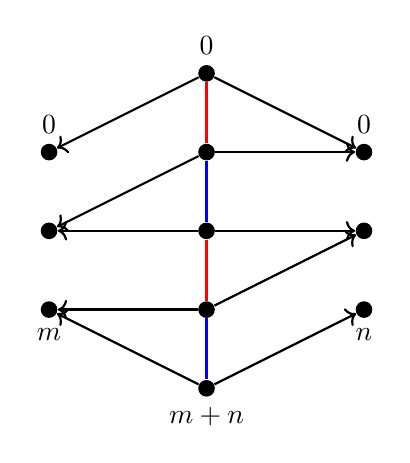
\begin{tikzpicture}[scale=1, transform shape]
            \node[label={north:{$0$}}, fill=black, circle,inner sep=0, minimum size=6pt] (a0) at (0,2) {};
            \node[label={south:{$m+n$}}, fill=black, circle,inner sep=0, minimum size=6pt] (a4) at (0,-2) {};
            \node[fill=black, circle, inner sep=0, minimum size=6pt] (a1) at (0,1) {};
            \node[fill=black, circle, inner sep=0, minimum size=6pt] (a2) at (0,0) {};
            \node[fill=black, circle, inner sep=0, minimum size=6pt] (a3) at (0,-1) {};
            \node[label={north:{$0$}}, fill=black, circle,inner sep=0, minimum size=6pt] (b0) at (-2,1) {};
            \node[label={south:{$m$}}, fill=black, circle,inner sep=0, minimum size=6pt] (b2) at (-2,-1) {};
            \node[fill=black, circle, inner sep=0, minimum size=6pt] (b1) at (-2,0) {};
            \node[label={north:{$0$}}, fill=black, circle,inner sep=0, minimum size=6pt] (c0) at (2,1) {};
            \node[label={south:{$n$}}, fill=black, circle,inner sep=0, minimum size=6pt] (c2) at (2,-1) {};
            \node[fill=black, circle, inner sep=0, minimum size=6pt] (c1) at (2,0) {};
            \draw[thick,->] (a0) -- (b0);
            \draw[thick,->] (a1) -- (b1);
            \draw[thick,->] (a3) -- (b2);
            \draw[thick,->] (a2) -- (b1);
            \draw[thick,->] (a4) -- (b2);
            \draw[thick,->] (a0) -- (c0);
            \draw[thick,->] (a1) -- (c0);
            \draw[thick,->] (a2) -- (c1);
            \draw[thick,->] (a3) -- (c1);
            \draw[thick,->] (a4) -- (c2);
            \draw[thick, red] (a0) -- (a1);
            \draw[thick, red] (a2) -- (a3);
            \draw[thick, blue] (a1) -- (a2);
            \draw[thick, blue] (a3) -- (a4);
        \end{tikzpicture}
        \end{center}
        \caption{A $(2,2)$ shuffle. Red lines denote where $\mu$ jumps and blue lines denote where $\nu$ jumps.}%
        \label{fig:22shuffle}
        \end{figure}
        We can see that an $(m,n)$-shuffle is simply a way to shuffle $m$ red and $n$ blue cards together. There is a unique permutation which takes the configuration having all red cards on top to our given shuffle.
    \end{itemize}
\end{defn}

\begin{prop}
    Let $R \in \ms{scRing}$. Then there is a map \(R_m \otimes R_n \xrightarrow{\cdot} R_{m+n}\) given by the formula
    \[ x \cdot y = \sum_{(\mu, \nu)} \on{sign}(\mu, \nu) s_{\mu}(x) s_{\nu}(y), \]
    where \(s_{\mu}(x)\) and \(s_{\nu}(y)\) correspond to applying the degeneracies making up $\mu$ and $\nu$ to obtain elements of $R_{m+n}$. This gives $R$ the structure of a strict cdga.
\end{prop}

\begin{proof}
    We will not go through all of the combinatorics explicitly.
    \begin{itemize}
        \item To prove associativity, we can express both \((xy)z\) and \(x(yz)\) as a sum
        \[ \sum_{(\lambda,\mu, \nu)}\on{sign}(\lambda, \mu, \nu) s_{\lambda}(x) s_{\mu}(y) s_{\nu}(z). \]
        \item To check commutativity, the fact that $R$ was a simplicial commutative ring means we can exchange the roles of $\mu$ and $\nu$ up to 
        \[ \frac{\on{sign}(\mu, \nu)}{\on{sign}(\nu, \mu)} = (-1)^{mn}, \]
        which is exactly what we desire.
        \item A variant of this argument also gives strictness. When we compute $x^2$, the summands corresponding to $(\mu, \nu)$ and $(\nu, \mu)$ appear with opposite signs, so we see that $x^2 = 0$.
        \item The differential is given by the alternating sum of the face maps. Applying this to $x \cdot y$ will decompose the result into $(m-1, n)$-shuffles and $(m, n-1)$-shuffles, which yields the desired result. \qedhere
    \end{itemize}
\end{proof}

We will now discuss divided power structures. In fact, every simplicial commutative ring will give us one of these.

\begin{prop}
    Let $R \in \ms{scRing}$ be a simplicial commutative ring. Then there exist maps $\gamma_k \colon R_n \to R_{nk}$ for all $n, k \geq 1$ such that
    \begin{itemize}
        \item We have $\gamma_1(x) = x$ for all $x \in R$;
        \item We also have 
        \[ \gamma_k(x) \gamma_{\ell}(x) = \binom{k+\ell}{\ell} \gamma_{k+\ell}(x) \] 
        for all $k, \ell$. This means that we should think that $x^k = k! \gamma_k(x)$;
        \item For all $x,y \in R_n$, we have
        \[ \gamma_k(x+y) = \sum_{i+k=k} \gamma_i(x) \gamma_j(y); \]
        \item Similarly, we have
        \[ \gamma_k(xy) = x^k \gamma_k(y); \]
        \item We have the identity
        \[ \gamma_k (\gamma_{\ell}(x)) = \frac{(k\ell)!}{k! (\ell!)^k} \gamma_{k\ell}(x). \]
    \end{itemize}
\end{prop}

\begin{proof}
    If $x$ is odd, we define $\gamma_1(x) = x$ and $\gamma_k(x) = 0$ for all $k \geq 2$. This is fine because $x^2 = 0$ already. If $x$ is even, we have
    \[ x^k = \sum_{(\mu_1, \ldots, \mu_k)} \on{sign}(\mu_1, \ldots, \mu_k) s_{\mu_1}(x) \cdots s_{\mu_k}(x). \]
    We can permute the factors $\mu_1, \ldots, \mu_k$ (all of the signs will become $+1$), and therefore for all $\sigma \in \Sigma_k$, $(\mu_1, \ldots, \mu_k)$ and $(\mu_{\sigma(1)}, \ldots, \mu_{\sigma(k)})$ give the same summand. Choosing one element from each equivalent class, we obtain an element $\gamma_k(x)$ such that $x^k = k! \gamma_k(x)$.

    We will omit checking that the properties are satisfied.
\end{proof}

We now need to make sure that this divided power structure behaves well with respect to the chain differential.
\begin{prop}
    Let $R \in \ms{scRing}$ be a simplicial commutative ring. Then
    \begin{itemize}
        \item If $x$ is even, then $\d{\gamma_k(x)} = \gamma_{k-1}(x)\cdot \d{x}$;
        \item The maps $\gamma_k$ preserve boundaries;
        \item The $\gamma_k$ give a well-defined divided power structure on $H_*(R)$.
    \end{itemize}
\end{prop}

\begin{proof}
    Suppose that $x$ is a boundary. Then $x = \d{y}$ for $x$ with $\d_i y = 0$ for all $i > 0$. Define
    \[
        \gamma_k'(y) \coloneqq \sum_{\substack{(\mu_1, \ldots, \mu_k) \\ \Sigma_k \text{-representatives}}} \on{sign}(\mu_1, \ldots, \mu_k) s_{\mu_1'}(y) \cdots s_{\mu_k'}(y).
    \]
    Here, for maps $\mu_i \colon [kn] \to [n]$, we set $\mu_i' \colon [1+kn] \to [1+n]$ to be the maps given by sticking a $1$ in front. Then $\d_0 \gamma_k'(y) = \gamma_k(x)$ and $\d_i \gamma_k'(y) = 0$ for all $i > 0$, and therefore $\d{\gamma_k'(y)} = \gamma_k(x)$.
\end{proof}

\end{document}

%%% Local Variables:
%%% mode: latex
%%% TeX-master: t
%%% End:
